% One patch in feature space (Propositions 1-3). Drawn at ~print size for 0.47\linewidth: labels are direct (no legend),
% circled numbers link each path to its proposition.
\documentclass[tikz,border=1pt]{standalone}
\usepackage[T1]{fontenc}
\usepackage{times}
\usepackage{amsmath,amssymb,bm}
\usetikzlibrary{arrows.meta,calc,shapes.geometric}
\definecolor{ink}{HTML}{1F2A37}
\definecolor{subink}{HTML}{5B6573}
\definecolor{obsblue}{HTML}{52627A}% observed features: neutral slate (blue = Direct)
\definecolor{oursgreen}{HTML}{009E73}
\definecolor{gateamber}{HTML}{E69F00}
\definecolor{addred}{HTML}{0072B2}% additive head = the Direct baseline (Direct blue)
\definecolor{arorange}{HTML}{D55E00}
\newcommand{\z}{\mathbf{z}}
\tikzset{badge/.style={circle, fill=#1, text=white, font=\scriptsize\bfseries, inner sep=0.5pt, minimum size=10.5pt}}
\begin{document}
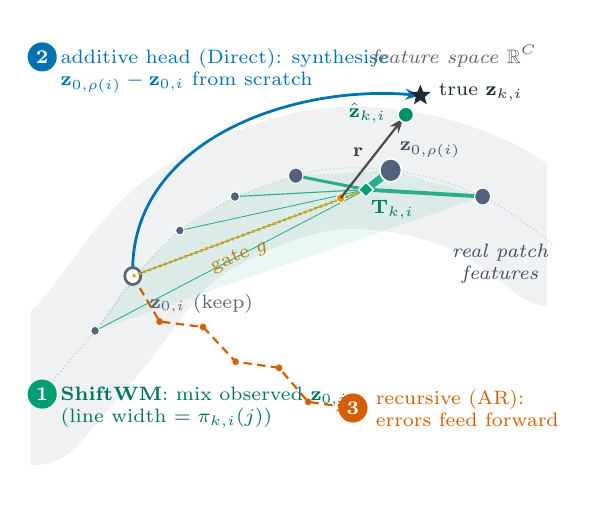
\begin{tikzpicture}[font=\scriptsize, >={Stealth[length=1.9mm,width=1.4mm]}]
\fill[white] (0,0) rectangle (6.6,5.75);
\node[anchor=north east, font=\scriptsize\itshape, text=subink] at (6.55,5.65) {feature space $\mathbb{R}^{C}$};
\begin{scope}[x=0.92cm, y=0.98cm, shift={(-0.62cm,-0.55cm)}]
  \def\band{plot[smooth, tension=0.6] coordinates {(0.7,1.55) (1.56,2.5) (2.73,3.8) (4.33,4.51) (5.64,4.58) (6.91,4.24) (7.9,3.6)}}
  \begin{scope}\clip (0.67,0.56) rectangle (7.8,6.3);
    \draw[line width=1.55cm, obsblue!9, line cap=round] \band;
  \end{scope}
  \draw[obsblue!35, line width=0.4pt, densely dotted] \band;
  \node[font=\scriptsize\itshape, text=obsblue!80!black, anchor=north, align=center] at (7.15,3.75) {real patch\\features};

  \coordinate (zi) at (2.08,3.21); \coordinate (p1) at (1.56,2.5); \coordinate (p2) at (2.73,3.8);
  \coordinate (p3) at (3.49,4.24); \coordinate (p4) at (4.33,4.51); \coordinate (pi) at (5.64,4.58);
  \coordinate (p6) at (6.91,4.24);
  \coordinate (T)  at (5.3,4.33);
  \coordinate (zg) at (4.95,4.22);
  \coordinate (zt) at (6.05,5.55);
  \coordinate (zh) at (5.85,5.3);

  \fill[oursgreen, opacity=0.08] (p1) -- (zi) -- (p2) -- (p3) -- (p4) -- (pi) -- (p6) -- cycle;
  \foreach \p/\w in {p1/0.3, zi/0.3, p2/0.3, p3/0.4, p4/1.1, pi/2.6, p6/1.4}{\draw[oursgreen, line width=\w pt, opacity=0.8] (\p) -- (T);}
  \draw[->, addred, line width=1.0pt] (zi) to[out=92, in=175] (zt);
  \node[font=\scriptsize, text=addred, anchor=north west, align=left] at (0.95,6.28)
    {additive head (Direct): synthesise\\$\z_{0,\rho(i)}-\z_{0,i}$ from scratch};
  \draw[arorange, line width=0.8pt, densely dashed, ->] (zi) -- (2.45,2.62) -- (3.05,2.55) -- (3.5,2.1) -- (4.1,2.02) -- (4.5,1.58) -- (5.1,1.5);
  \foreach \q in {(2.45,2.62),(3.05,2.55),(3.5,2.1),(4.1,2.02),(4.5,1.58)}{\fill[arorange] \q circle (0.045);}
  \node[font=\scriptsize, text=arorange, anchor=west, align=left] at (5.3,1.5) {recursive (AR):\\errors feed forward};
  \foreach \p/\r in {p1/0.06, p2/0.06, p3/0.065, p4/0.1, p6/0.11}{\fill[obsblue, draw=white, line width=0.4pt] (\p) circle (\r);}
  \fill[obsblue, draw=white, line width=0.6pt] (pi) circle (0.15);
  \draw[subink, line width=1pt, fill=white] (zi) circle (0.11);
  \node[font=\scriptsize, text=subink, anchor=north west] at ($(zi)+(0.1,-0.1)$) {$\z_{0,i}$ (keep)};
  \node[font=\scriptsize, text=obsblue!85!black, anchor=south west, inner sep=1pt] at ($(pi)+(0.08,0.12)$) {$\z_{0,\rho(i)}$};
  \draw[gateamber, line width=1pt, densely dotted] (zi) -- (T);
  \node[font=\scriptsize, text=gateamber!80!black, anchor=north, rotate=22, inner sep=1pt] at ($(zi)!0.42!(T)+(0.06,-0.08)$) {gate $g$};
  \fill[gateamber, draw=white, line width=0.3pt] (zg) circle (0.06);
  \draw[->, black!70, line width=0.8pt, shorten >=1.5pt] (zg) -- (zh);
  \node[font=\scriptsize, text=black!75, anchor=east] at ($(zg)!0.55!(zh)+(-0.05,0)$) {$\mathbf{r}$};
  \node[diamond, fill=oursgreen, draw=white, line width=0.5pt, inner sep=1.4pt] at (T) {};
  \node[font=\scriptsize, text=oursgreen!80!black, anchor=north west, inner sep=1pt] at ($(T)+(0.02,-0.1)$) {$\mathbf{T}_{k,i}$};
  \node[circle, fill=oursgreen!90!black, draw=white, line width=0.6pt, inner sep=2pt] at (zh) {};
  \node[star, star points=5, star point ratio=2.3, fill=ink, inner sep=1.2pt] at (zt) {};
  \node[font=\scriptsize, text=ink, anchor=west] at ($(zt)+(0.12,0.04)$) {true $\z_{k,i}$};
  \node[font=\scriptsize\bfseries, text=oursgreen!75!black, anchor=east] at ($(zh)+(-0.14,0.02)$) {$\hat{\z}_{k,i}$};
  \node[font=\scriptsize, text=oursgreen!75!black, anchor=north west, align=left] at (0.95,1.9)
    {\textbf{ShiftWM}: mix observed $\z_{0,j}$\\(line width $=\pi_{k,i}(j)$)};
  \node[badge=oursgreen] at (0.83,1.68) {1};
  \node[badge=addred] at (0.83,6.05) {2};
  \node[badge=arorange] at (5.12,1.5) {3};
\end{scope}
\end{tikzpicture}
\end{document}
